\part{Cuarto semestre}

\chapterimage{5.pdf} % Chapter heading image


\chapter{Métodos Numéricos}

\section{Introducción}
\subsection{Conceptos}
\begin{definition}[Métodos numéricos]
    son técnicas mediante las cuales es posible formular problemas de tal forma, que puedan resolverse usando Operaciones Aritméticas (Chapra, 1977).
\end{definition}
Existen muchos tipos de Métodos Numéricos, sin embargo, todos comparten una característica común; todos llevan a cabo un número TEDIOSO de cálculos aritméticos.

Los Métodos Numéricos se han desarrollado con el objetivo de resolver problemas matemáticos, cuya solución es difícil o "imposible" de obtener por los métodos tradicionales. Es una secuencia de operaciones algebraicas y lógicas que producen la aproximación al problema matemático con una Tolerancia o Error máximo permitido o predeterminado.

Se clasifican en métodos directos e iterativos.

\subsubsection{Métodos Directos}
Tienen una secuencia de pasos definidos, que conducen a la solución del problema; por lo regular la solución se obtiene en forma analítica.

\subsubsection{Métodos Iterativos}

En éstos se parte de una solución inicial y mediante aplicación de un algoritmo específico, se van obteniendo aproximaciones a la solución del problema.

En éstos métodos se repite una serie de pasos y se basan en la aplicación de las llamadas ecuaciones de recurrencia, las cuales relacionan dos o más elementos consecutivos de una sucesión de números, funciones ó matrices.

\begin{definition}[Sucesión numérica]
    Es una lista de números cuyo origen es el mismo, es decir, son el resultado de aplicar una serie de pasos que se repiten en un algoritmo. A esta serie de pasos se les denomina Iteración.
\end{definition}
\section{Localización de raíces de ecuaciones}
\subsection{Métodos Iterativos o Abiertos}

La solución de las ecuaciones no lineales es difícil y en muchas ocasiones no hay forma analítica de encontrar la solución de estas. Sin embargo, se puede realizar a través de un proceso iterativo; partir de una solución inicial y a través de un proceso algebraico repetitivo, obtener una solución mejorada a la solución anterior.
\subsection{Raíces de Ecuaciones No Lineales}
La solución de este tipo de métodos implica 2 pasos fundamentales:
\begin{enumerate}
    \item Acotar la solución.
    \item Mejorar a través de un proceso iterativo la solución anterior. Para el primer paso se deberá tomar en cuenta lo siguiente:
    \begin{enumerate}
        \item Una Búsqueda sistemática.
        \item Experiencia en problemas anteriores, similares o semejantes.
        \item Conocer la solución de un modelo simplificado y usarla como punto de partida, es decir, usarla como solución inicial.
        \item La solución anterior será una secuencia de soluciones
    \end{enumerate}
\end{enumerate}

Los métodos usados para este tipo de ecuaciones son:
\begin{itemize}
    \item Método de la Bisección.
    \item Método del Punto Fijo.
    \item Método de Newton-Raphson.
    \item Método de la Secante.
\end{itemize}

\subsection{Método de la Bisección}
El método parte de una función F(X) y un intervalo $[x_1,x_2]$ tal que $F(x_1)$ y $F(x_2)$ tienen signos contrarios. Si la función es continua en este intervalo, entonces existe una raíz de $F(X)$ entre $x_1$ y $x_2$.

Una vez determinado el intervalo $[x_1,x_2]$ y asegurada la continuidad de la función en dicho intervalo, se evalúa esta en el punto medio Xm del intervalo. Si $F(x_m)$ y $F(x_1)$ tienen signos contrarios, se reducirá el intervalo de $x_1$ a $x_m$, ya que dentro de estos valores se encuentra la raíz buscada. Al repetir este proceso, hasta lograr que la diferencia entre los dos últimos valores de $x_m$ sea menor que una tolerancia prefijada, el último valor Xm será una buena aproximación de la raíz.


\subsection{Método de Newton-Raphson}
Se debe tener idea de la solución, es decir el valor inicial es muy importante.
Recordando la ecuación de recursión de Newton-Raphson:
\begin{equation}
    x_1= x_0\frac{f(x_0)}{f^{\prime}(x)}
\end{equation}
No se debe perder de vista que la tolerancia $\xi$, la cuál es: $\left\lvert x_{i+1}-x_i \right\rvert  \leq \xi$
En no más de diez iteraciones, la gráfica converge,
\begin{example}
    Resolver la siguiente ecuación por Newton-Raphson:
    Con $\xi=0.001$:
    \begin{equation*}
        f(x)= \sqrt{x}=x^{\frac{1}{2}}
    \end{equation*}
\end{example}

\textit{ Sol. }

La propuesta inicial va a ser: $x_0=x$, por lo tanto aplicando la formula:
\begin{align*}
    &x_{i + 1 }= x_i - f\frac{x_i}{f^{\prime}(x_i)}\\
    &f^{\prime}(x_i) = \frac{1}{2}x^{\frac{1}{2}} = \frac{1}{2x^{\frac{1}{2}}}\\
    &x_1 = x_{0} - 2x^{\frac{1}{2}}\cdot x^{\frac{1}{2}}\\
    &\therefore x_1= - x_0
\end{align*}
Gráficamente se vería de la siguiente forma:
\begin{figure}[h!]
\centering
  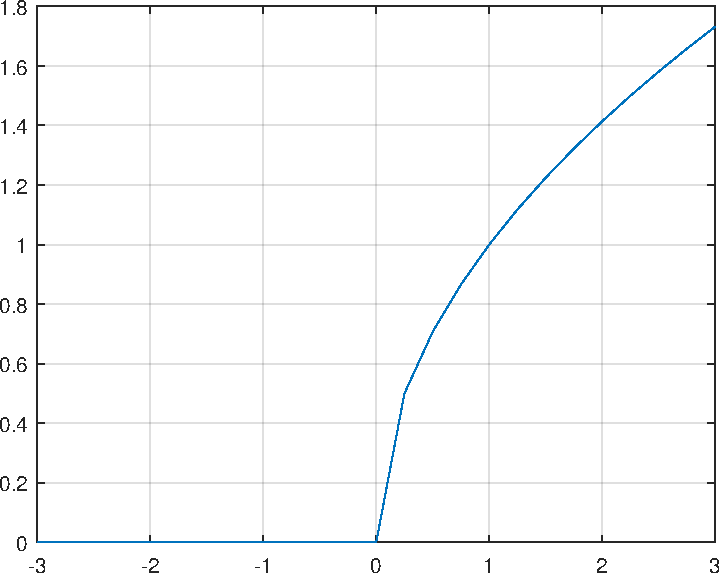
\includegraphics[width=0.5\textwidth]{mn2.pdf}
  \caption{Esquema de la solución}
  \label{mn2}
\end{figure}
El Algoritmo para el método de Newton Raphson con pseudocódigo sería como sigue:
\begin{lstlisting}
    salir <- 0
    int i<-0
    Mientras (i<= MoIterMax) y (salir==0) haz
    {
        x1=x0-f(x0)/df(x0)
        si (f(x1)==0) o (abs(x1-x0)<=Tolerancia) Entonces{
            Escribir("Llegue a la solucion en",i,"iteraciones")
            Escribir("xsd:",x1)
            exit
        }
    De otra forma{
        i<- i+1
        x0<-x1
    }
    }
    if(i>=NoITerMax) entonces
    Escribe("El metodo fallo: cambie de metodo")
\end{lstlisting}
La entrada que se le debe dar a los comandos son:
\begin{lstlisting}
    funcion f(x)d
    funcion df(x)
    float x0
\end{lstlisting}
La salida debe ser $x1<- float$:

\begin{lstlisting}
    A=10
    B=20
    C=A+B
    print('C: ', C)
    
    def f(x):
        return (x**2)-(2*x)-3
    def df(x):
        return (2*x)-2
    
    NoIterMax=100
    Tolerancia=0.000001
    x0=-0.5
    Salir=0
    i=0
    while (i<=NoIterMax) and (Salir==0):
        x1=x0-(f(x0)/df(x0))
        print('x0:', x0, 'f(x0)', f(x0), ' df(x0)', df(x0), 'x1: ', x1)
        if (((x1)==0) or (abs(x1-x0)<=Tolerancia)):
            print("Solucion en",i,"Iteraciones")
            print("xsol=",x1)
            Salir=1
        else:
            i=i+1
            x0=x1
        if (i>=NoIterMax):
            print("El metodo fallo: cambie de metodo")
    \end{lstlisting}
    Éste método es descrito por la figura \ref{mn3}
\begin{figure}[h!]
\centering
  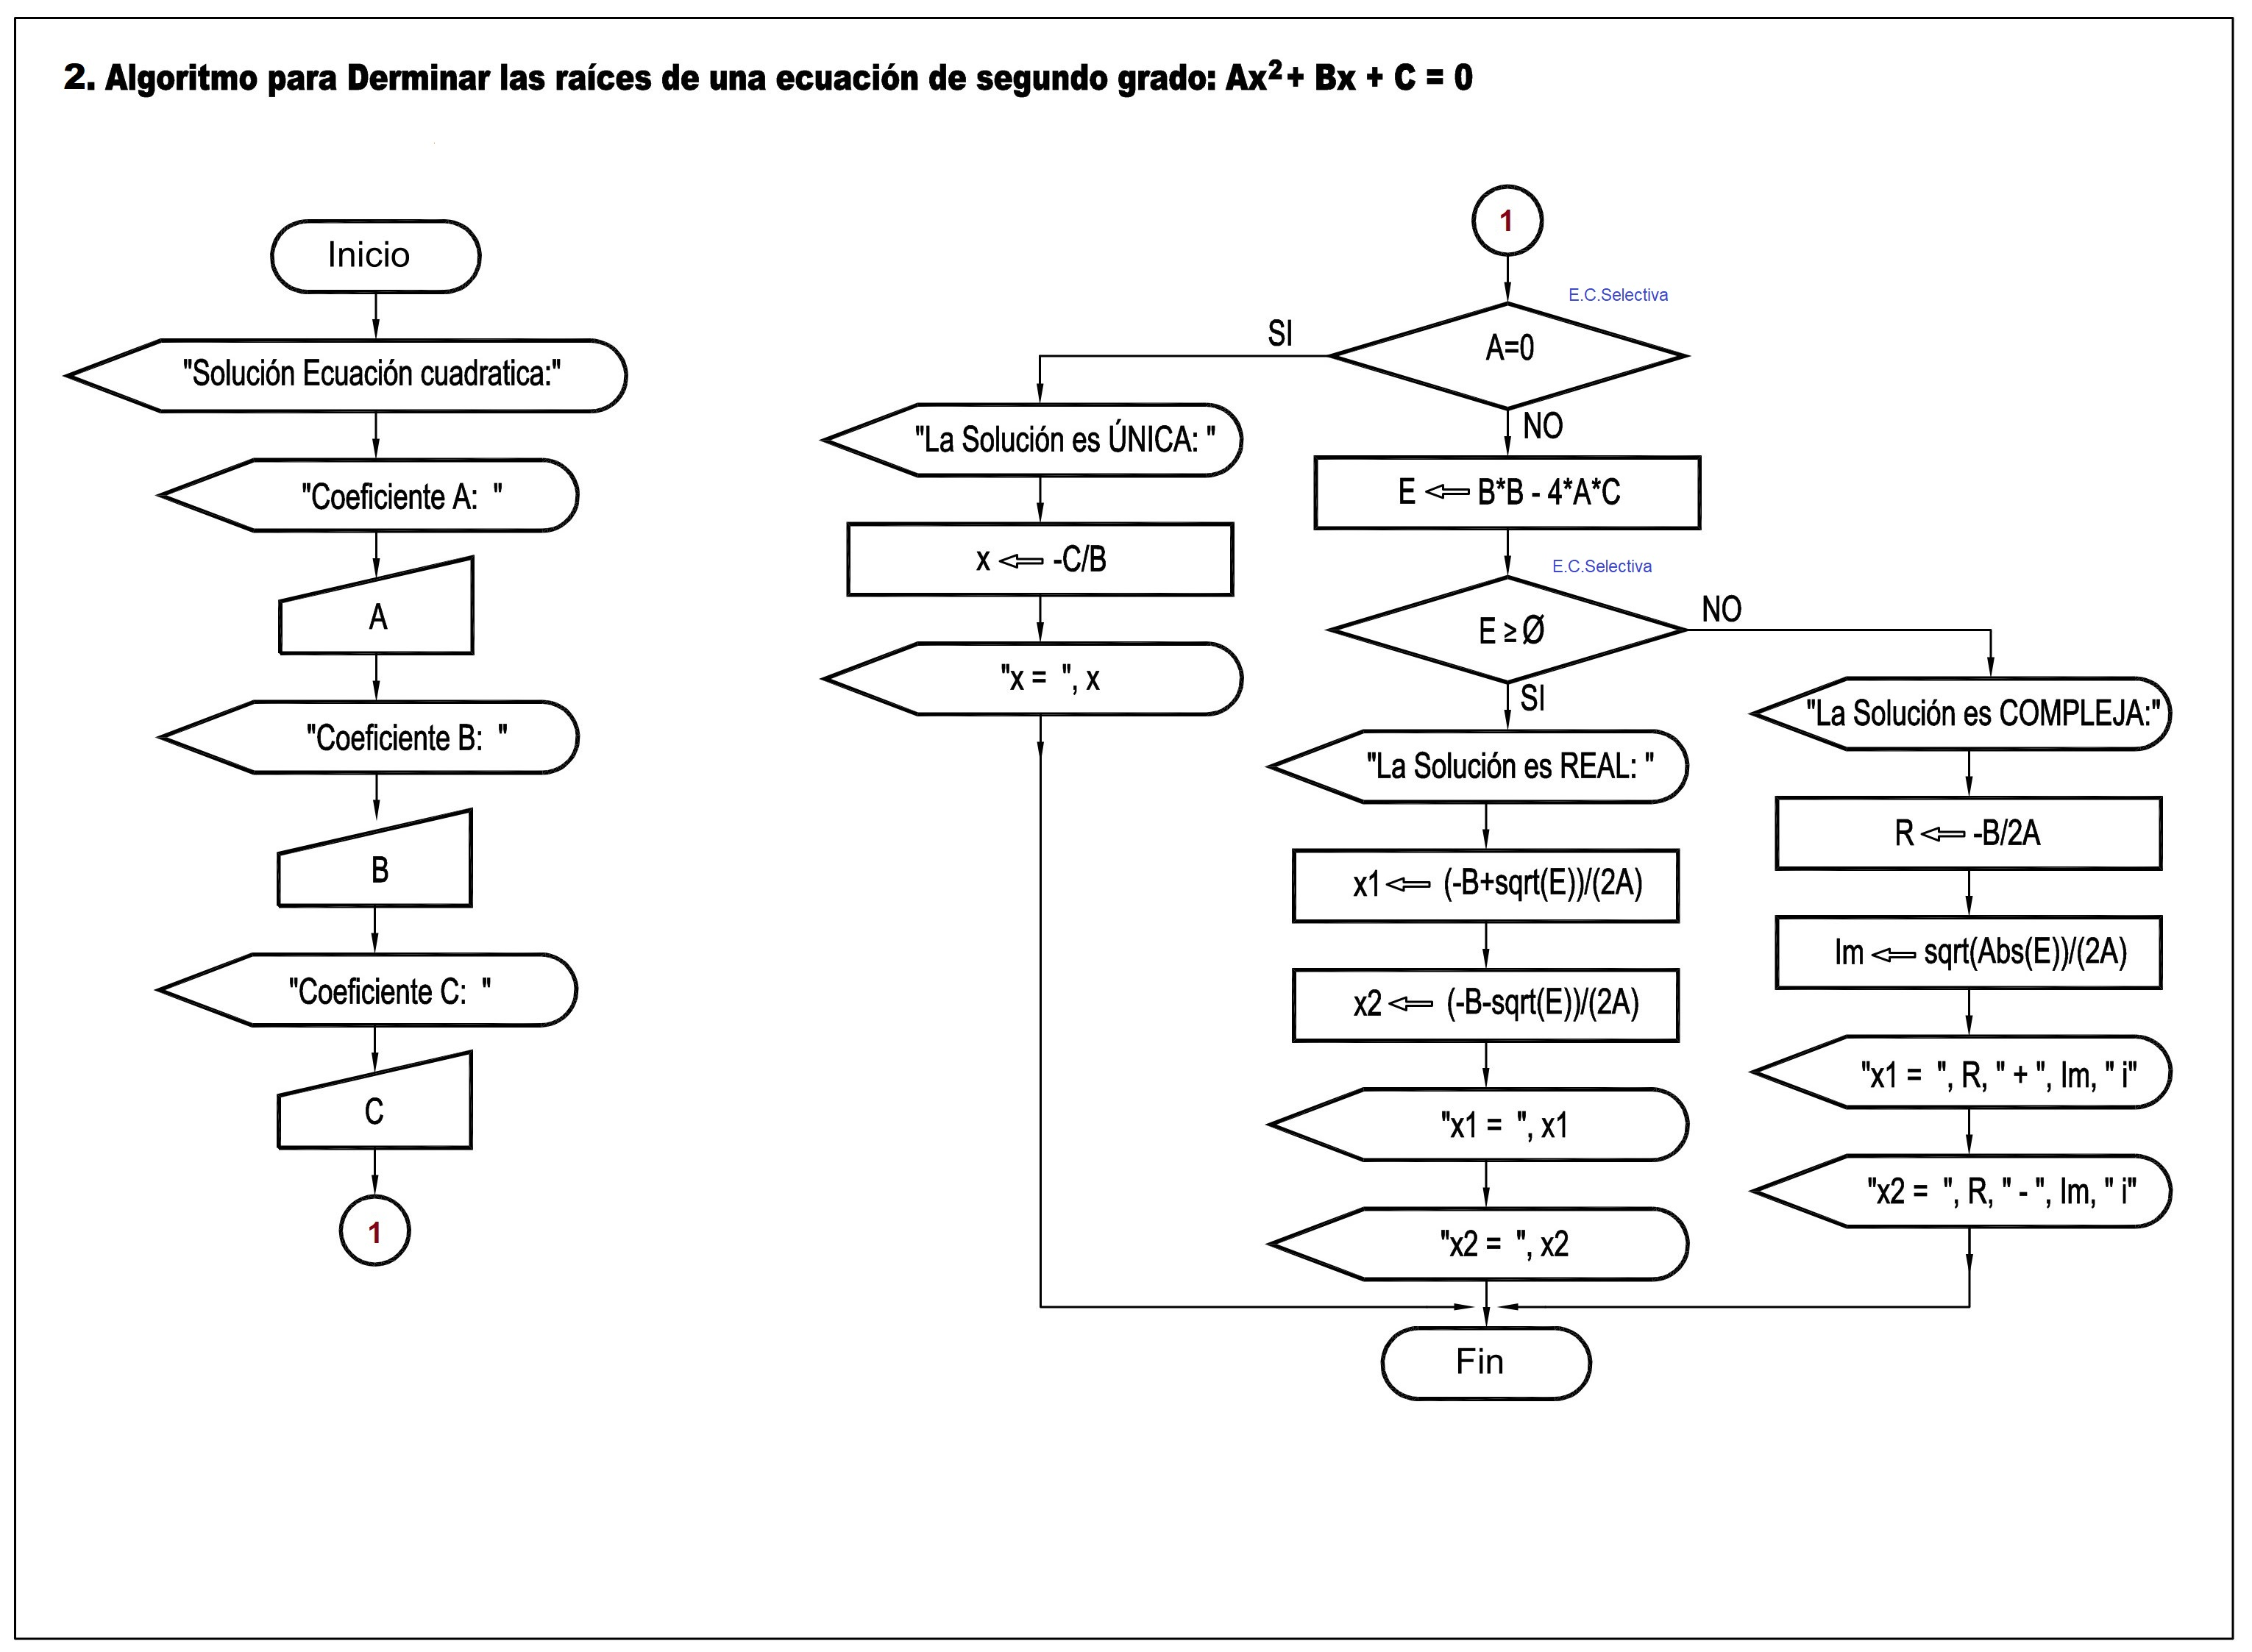
\includegraphics[width=0.5\textwidth]{mn3.jpg}
  \caption{Algoritmo de la ecuación cuadrada}
  \label{mn3}
\end{figure}
    Nótese que $x(i+1)$ será una mejor aproximación que $x(i)$, $x(i)$ una mejor aproximación que $x(i+1)$. La propuesta inicial es que x(i) sea x1 y la siguiente $x(i+1)=x2$.
    La ecuación de recurrencia de la Secantes es:
    % \begin{equation}
    %     x_2 = x_1 -\left\{\right\}
    % \end{equation}
    Recordando la fórmula cuadrática $Ax^2+Bx+C=0$, entonces sí A=0, entonces: $Bx+C=0$, 
    $x=-\frac{C}{B}$, de otra forma: $x=\frac{-B\pm\sqrt{B^2-4AC}}{2A}$.
    Asignando la variable $E: B^2-4AC$, sí $E\leq 0$ entonces:
    \begin{align*}
        &X_1 = \frac{-B\pm\sqrt{B^2 +4AC}}{2A}\\
        &X_2 = \frac{-B\pm\sqrt{B^2-4AC}}{2A}
    \end{align*}
    Es deci, tiene solución real, de otra forma:
    \begin{align*}
        &X = \frac{-B\pm\sqrt{B^2-4AC}}{2A}\\
        &\implies X = \frac{- B}{2A}\pm\frac{\sqrt{B^2+4AC}}{2A}
    \end{align*}
    (La solución se conforma de una parte real e imaginaria):
    \begin{equation*}
        X = \mathbb{R} \pm I_m
    \end{equation*}
    \begin{lstlisting}[language=Python]
        import math
    
    A = float(input('Coeficiente A: '))
    B = float(input('Coeficiente B: '))
    C = float(input('Coeficiente C: '))
    
    if A==0: 
        print ('la solucion es lineal')
        x = -C/B
        print ('x = ',x)
    else:
        E = B**2-4*A*C
        if E>=0:
            print('la solucion es real')
            x1 = (-B+math.sqrt(E))/(2*A)
            x2 = (-Bmath.sqrt(E))/(2*A)
            print('x1 = ',x1,'x2 = ',x2)
        else: 
            print('la solucion es compleja')
            R = -B/(2*A)
            Im = math.sqrt(abs(E))/(2*A)
            print ('x1 = ',complex(R,Im))
            print ('x2 = ',complex(R,-Im))
            print ('x1 = ',R,'+',Im,'i')
            print ('x2 = ',R,'-',Im,'i')
    \end{lstlisting}
Otro ejemplo es dado por:
\begin{lstlisting}
    n = int(input('Dame un numero: '))
rana = 0
while rana < n:
    rana += 2
if rana == n:
    print('El numero es par')
else: 
    print('El numero es impar')
\end{lstlisting}
\subsection{Método de Gauss-Seidel}
Los métodos iterativos constituyen una alternativa a los métodos de eliminación descritas hasta ahora para aproximar la solución. Tales métodos son similares a las técnicas que se desarrollaron para obtener las raíces de una ecuación. Aquellos métodos consistían en suponer un valor y luego usar un método sistemático para obtener una aproximación mejorada de la raíz. Como esta parte trata con un problema similar (obtener los valores que simultáneamente satisfagan un conjunto de ecuaciones). Entonces se esperaría que tales métodos aproximados fuesen útiles en este contexto.

El método de Gauss-Seidel es el más común, suponga un sistema de $n$ ecuaciones:
\begin{equation}
    [A][X] =[B]
\end{equation}
Suponga que se limita a un conjunto de ecuaciones 3x3, si la diagonal no son cero, la primera ecuación se puede resolver para $x_1$, la segunda para $x_2$ y la tercera $x_3$ para obtener:
\begin{align*}
    &x_1 =\frac{b_1 - a_{12}x_2 - a_{13}x_3}{a_{11}}\\
    &x_2 =\frac{b_2 - a_{21}x_1 - a_{23}x_3}{a_{22}}\\
    &x_3 =\frac{b_3 - a_{31}x_1 - a_{32}x_2}{a_{33}}
\end{align*}
Ahora escogiendo los valores iniciales para las $x$, una forma simple para obtener los valores iniciales es suponer que todos son cero. Estos ceros se sustituyen en la ecuación (1a), la cual se utiliza para calcular un nuevo valor $x_1=\frac{b_1}{a_{11}}$. Después se sustituye este nuevo valor de $x_1$ junto con el valor previo cero de $x_3$ en la ecuación de $x_2$. Este proceso se repite con la ecuación de $x_3$. Después se regresa a la primera ecuación y se repite todo el procedimiento hasta que la solución converja suficientemente cerca a los valores verdaderos. La convergencia se verifica usando el criterio.
\begin{equation}
\left\lvert \epsilon_{a,i}\right\rvert = \left\lvert \frac{x_i^j - x_i^{j - 1}}{x_i^j}\right\rvert\cdot 100\%  
\end{equation}
Para todas las $i$, donde $j$ y $j-1$ son las iteraciones actuales y previas, respectivamente.

\subsection{Método de Jacobi}

Este es un método alternativo, emplea una táctica usando las mismas ecuaciones despejadas del método de Gauss-Seidel para calcular un conjunto de nuevas x con base en un conjunto de x anteriores. De esta forma conforme se generan nuevos valores, no se usan de forma inmediata, se retienen para la siguiente iteración.

La diferencia entre el método de Gauss-Seidel y el de la iteración de Jacobi es descrito en el siguiente esquema:

En la primera iteración:
\begin{align*}
    x_1 = \frac{\left(b_1 - a_{12}x_2 - a_{13}x_3 \right)}{a_{11}} && x_1 = \frac{\left(b_1 - a_{12}x_2 - a_{13}x_3 \right)}{a_{11}}\\
    x_2 = \frac{\left(b_2 - a_{21}x_1 - a_{23}x_3 \right)}{a_{22}}&& x_2 = \frac{\left(b_2 - a_{21}x_1 - a_{23}x_3\right)}{a_{22}}\\
    x_3 = \frac{\left(b_3 - a_{31}x_1 - a_{32}x_2\right)}{a_{33}} && x_3 = \frac{\left(b_3 - a_{31}x_1 - a_{32}x_2\right)}{a_{33}}
\end{align*}
Segunda iteración:
\begin{align*}
    x_1 = \frac{\left(b_1 - a_{12}x_2 - a_{13}x_3 \right)}{a_{11}} && x_1 = \frac{\left(b_1 - a_{12}x_2 - a_{13}x_3 \right)}{a_{11}}\\
    x_2 = \frac{\left(b_2 - a_{21}x_1 - a_{23}x_3 \right)}{a_{22}}&& x_2 = \frac{\left(b_2 - a_{21}x_1 - a_{23}x_3\right)}{a_{22}}\\
    x_3 = \frac{\left(b_3 - a_{31}x_1 - a_{32}x_2\right)}{a_{33}} && x_3 = \frac{\left(b_3 - a_{31}x_1 - a_{32}x_2\right)}{a_{33}}
\end{align*}

Del lado izquierdo es el método de Gauss-Seidel y del lado derecho es el método de Jacobi.

\section{Diferenciación e integración numérica}

\subsection{Fórmulas de Newton-Cotes para la ingeniería numérica}

Son los tipos de integración numérica más comunes. Se basan en la estrategia de reemplazar una función complicada o datos tabulados por un polinomio de aproximación que es fácil de integrar:
\begin{equation}
    I = \int_a^b f(x)\, dx\cong \int_a^b f_n(x)\,dx
\end{equation}
Donde $F_n(x)$ es un polinomio de la forma:
\begin{equation}
    f_n = a_0 + a_1x +\dots +a_{n- 1}x^{n - 1} + a_n \cdot x^n
\end{equation}
Donde $n$ es el grado del polinomio. La integral se puede aproximar usando un conjunto de polinomios aplicados por pedazos a la función o datos, sobre segmentos de longitud constante; aunque pueden utilizarse polinomios de grado superior con los mismos propósitos. 

Existen formas cerradas y abiertas de las fórmulas de Newton-Cotes. Las formas cerradas son aquellas donde se conocen los datos al inicio y al final de los límites de integración. Las formas abiertas tienen límites de integración que se extienden más allá del intervalo de los datos.

Por lo general, las formas abiertas de Newton-Cotes no se usan para integración definida, pero para evaluar integrales impropias y para obtener la solución de ecuación diferenciales ordinarias.

\subsubsection{ La regla del trapecio}
Recordando, como se representa una línea recta: 
\begin{figure}[h!]
\centering
  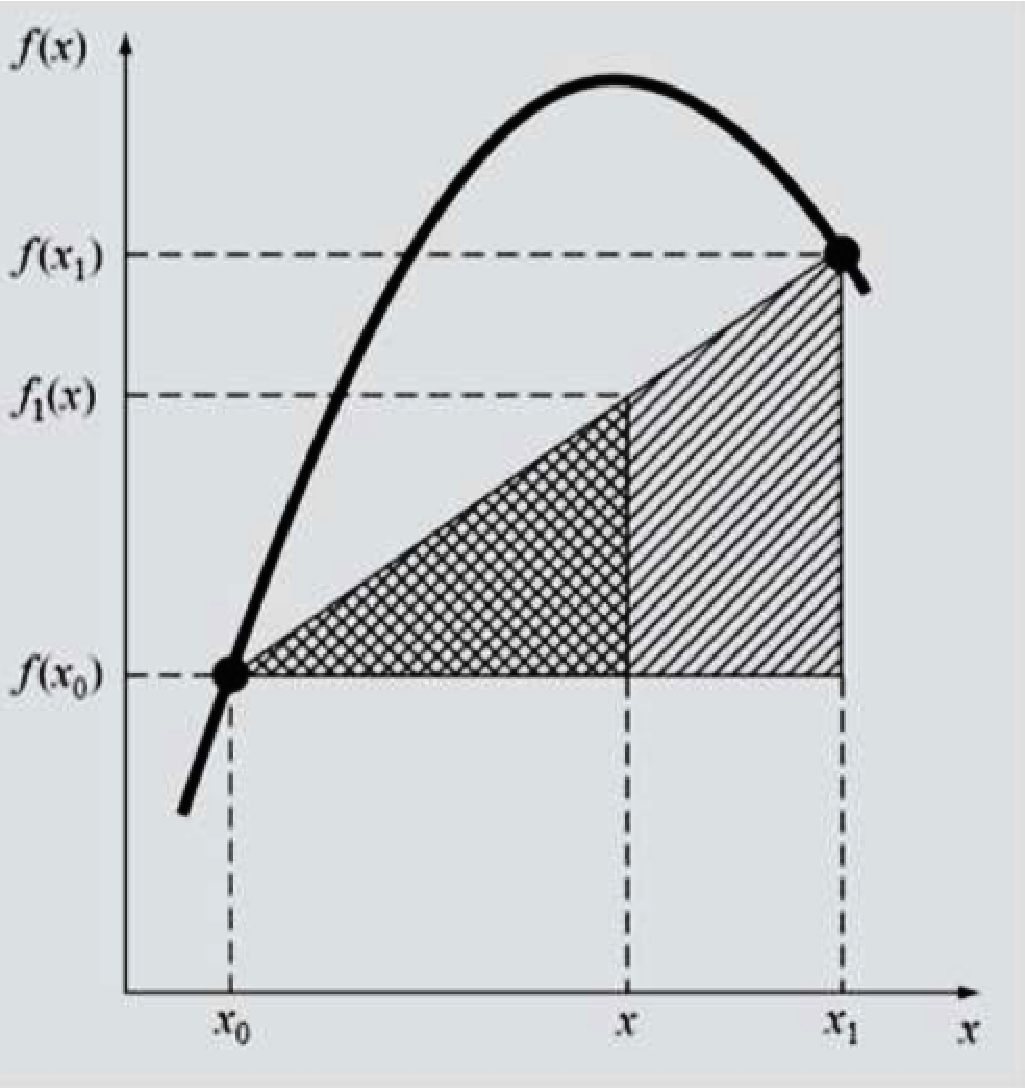
\includegraphics[width=0.5\textwidth]{mn4.pdf}
  \caption{Interpolación lineal, utilizando triángulos semejantes}
  \label{mn4}
\end{figure}
\begin{equation}
    \frac{f_1(x)- f(x_0)}{x -x_0} = 
\end{equation}

\section{Integración de Romberg}

Es una técnica diseñada para obtener integrales numéricas de funciones de manera eficiente. Es muy parecida a las técnicas analizadas, en el sentido de que se basa en aplicaciones sucesivas de la regla del trapecio. A través de las manipulaciones en los errores se alcanzan mejores resultados.

Hay técnicas de corrección del error para mejorar los resultados de la integración numérica con base en la misma estimación de la integración. Dichos métodos usan dos estimaciones de una integral para calcular una tercera más exacta y, en general, se les conoce como extrapolación de Richardson. 

La estimación y el error correspondiente a la regla del trapecio múltiple se representa de manera general como:
\begin{equation}
    I=I(h)+E(h)
\end{equation}
Donde $I$ es el valor de la integral, $I(h)$ la aproximación obtenida de una aplicación con $n$ segmentos de la regla del trapecio, con un tamaño de paso $h=\frac{b-a}{n}$ y $E(h)$ el error de truncamiento. SI hacemos, por separado dos estimaciones usando tamaños de paso $h_1$ y $h_2$ y tenemos valores exactos del error.
\begin{equation}
    I(h_1)+E(h_1)= I(h_2)+E(h_2)
\end{equation}
Ahora recuerde que el error de la regla del trapecio de aplicación múltiple puede representarse en forma aproximada mediante la ecuación con $n=(b-a)/h$
\begin{equation}
    E \approx \frac{b-a}{12}h^2f^{\prime\prime}
    \label{eqmn:error}
\end{equation}
Si se supone que $f^{\prime\prime}$ es constante para todo tamaño de paso, la ecuación se utiliza para determinar la razón entre los dos errores que será:
\begin{equation}
    \frac{E}{\frac{E(h_1)}{h_2}} =\frac{h_1^2}{h_2^2}
\end{equation}
Este cálculo tiene el importante efecto de eliminar el término $f^{\prime\prime}$ de los cálculos. Al hacerlo, fue posible utilizar la información contenida en la ecuación\eqref{eqmn:error} sin un conocimiento previo de la segunda derivada de la función. Para lograrlo se reordena la ecuación anterior para obtener:
\begin{equation}
    E(h_1) \approx E(h_2)\left(\frac{h_1}{h_2}\right)^2
\end{equation}
Se puede sustituir en la primera ecuación:
\begin{equation*}
    I(h_1) + E(h_2)\left(\frac{h_1}{h_2}\right)^2\approx I(h_2) + E(h_2)
\end{equation*}
Despejando obtuvimos:
\begin{equation}
    E(h_2) \approx \frac{I(h_1) -I(h_2)}{1 -\left(\frac{h_1}{h_2}\right)^2}
\end{equation}
Así, se estimó el error de truncamiento en términos de las estimaciones de la integral y de sus tamaños de paso. La estimación se sustituye después en $I=I(h_2)+E(h_2)$, entonces para obtener una mejor estimación de la integral:
\begin{equation}
    I \approx I(h_2) + \frac{1}{1 -\left(\frac{h_1}{h_2}\right)^2}\cdot\left(I(h_2) - I(h_1)\right)
\end{equation}
Se puede demostrar que el error de esta estimación es $O(h^4)$ combinando las dos estimaciones con la regla del trapecio de $O(h^2)$ para obtener una nueva estimación. En el caso donde el intervalo es dividido entre dos, se convierte en:
\begin{equation*}
    I \approx I(h_2) + \frac{1}{2^2- 1}\left(I(h_2) - I(h_1)\right)
\end{equation*}
Agrupando los términos:
\begin{equation}
    I \approx \frac{4}{3}I(h_2) - \frac{1}{3}I(h_1)
\end{equation}




